\documentclass{article}
\usepackage{amsmath}
\usepackage{graphicx}
\graphicspath{ {images/} }
\usepackage[section]{placeins}
\usepackage{titlesec}
\usepackage{enumitem}
\usepackage[hidelinks]{hyperref}

\newcommand{\sectionbreak}{\clearpage}
\titleformat{\paragraph}
{\normalfont\normalsize\bfseries}{\theparagraph}{1em}{}
\titlespacing*{\paragraph}
{0pt}{3.25ex plus 1ex minus .2ex}{1.5ex plus .2ex}

\newlist{RQ}{enumerate}{1}
\setlist[RQ]{label=RQ\arabic*:}

\setcounter{secnumdepth}{4}
\setcounter{tocdepth}{4}

\title{A study on user-centered design illustrated by development of social platform for dance classes attendees}
\author{Tomasz Legutko}
\date{2016/2017}
\begin{document}
\maketitle
% TODO document skeleton with frontpage from wiet
\tableofcontents
\section{Motivation}
Software development methodologies have always been and always will be an important part of all IT projects. With every year software becomes increasingly important part of our society and with every year the software's complexity becomes even harder to manage. Over the years there's been a great progress in architectural patterns, tools, best practices and particularly, development methodologies and frameworks.

Historically speaking, software development methodologies have come a really long way from sequential, plan driven to more lightweight, iterative approaches gathered under the common name ``Agile'', nowadays applied by and large in the industry. But as there are no silver bullets, agile methods have their limitations and can benefit greatly from extensions.

Approaches gathered under the domain of Human-Computer Interface, particularly User Centered Design were recognized by researchers to be complementary to Agile shortcomings and there were a lot of scientific effort to combine those methods and provide patterns and guidelines for practitioners. 

One important area, where those practices cannot be easily applied is in startups, that is newly found software companies with little to none operating history, operating with lack of resources under extreme time pressure to quickly create product and find appropriate market for it. To answer needs for specific approach, Eric Ries proposed Lean Startup approach.

But as Agile could benefit from User Centered Design practices, so could Lean Startup, and the scientific effort in this area resulted in Lean UX approach. But the research on this topic is scarce and in an attempt fill the gap author decided to perform case study of his own startup in the light of Lean UX advices in order to present lessons learned and provide guidelines for industry practitioners.

\section{Introduction}
\subsection{Brief history of software development process}
Nowadays, agile methods are without a doubt an IT industry standard. But many think of them as just a replacement for waterfall, while iterative and incremental development dates as back as to mid-1950s, with few well documented undertakings by IBM and NASA \cite{larman2003iterative}.

\subsubsection{Waterfall}
Waterfall became well-known after 1970 Winston Royce's article ``Managing the Development of Large Software Systems''. It promoted well-defined, strict process, consisting of gathering requirements, analysis, design, coding, testing and maintaining. Even though original article advised following those activities twice, waterfall was most known as it's single-pass version and became a standard for long years, especially in large-scale and enterprise projects. Craig Larman \cite{larman2003iterative} argues that, as famous H.L.Mecken quote says ``For every complex problem, there is a solution that is simple, neat and wrong.'', waterfall gave illusory sense of ``orderly, accountable, and measurable process, with simple, document-driven milestones'', was easy to explain and recall (much easier than iterative and incremental development practices already present at that time) and widely promoted in literature.

\subsubsection{Iterative and incremental development methodologies}
Back in 1970s iterative and incremental development (IID) approach was already becoming recognized as more natural and fitting to manage projects than waterfall, notably IID incorporation by IBM Trident submarine system with above 1 million lines of code and NASA's space shuttle software. In 1976 ``Software Metrics'' Tom Glib proposed ``evolutionary project management'', and argued that system should be implemented in small steps, producing the appearance of stability in order to ``have opportunity of receiving some feedback from the real world before throwing in all resources intended for a system''.

1980s consisted of vast amount of criticism in literature towards unquestioned dominance of waterfall in industry \cite{larman2003iterative}, advocating IID approach, with notable 1985 Barry Boehm's publication ``A Spiral Model of Software Development and Enhancement''. It introduced risk assessment and project review in each iteration along with development phase using appropriate management model. During that time there were well documented significant project failures by US Department of Defense using document-driven waterfall approach, which resulted in adjusting formal standards (DoD-Std-2167A) to encourage usage of IDD.

In 1990s, software development industry was much more aware of IID practices and there were many books, articles and standards promoting IID. In second half of 1990s most currently known methodologies were created - Scrum, eXtreme Programming (XP), Lean Software Development, Rational Unified Process, Dynamic Systems Development Method and Feature Driven Development.

In 2001, a group of 17 methodologies experts, including all of above mentioned met in Utah to discuss common practices and the term ``Agile'' was coined.

\subsubsection{Reigns of Agile}

Meeting in 2001 resulted in famous Agile Manifesto \cite{beck2001agile}:
\begin{itemize}
  \item Individuals and interactions over processes and tools
  \item Working software over comprehensive documentation
  \item Customer collaboration over contract negotiation
  \item Responding to change over following a plan
\end{itemize}

Agile clearly promotes lightweight process and has been well received in industry and increasingly adopted, with recent 11th Annual State of Agile Report in 2017 \cite{one201711th} stating that over 94\% of over 20,000 respondents claimed their organizations practiced agile.

Since the creation of agile, the industry has also moved forward by leaps and bounds in technical areas. Automation is now common in software process - quality assurance, continuous integration and continuous delivery, internet as development environment, distribution means and execution infrastructure. Not to mention great progress in languages, tools, frameworks and architectural solutions. \cite{fuggetta2014software}
The progress is unquestionable and although large IT projects were once notorious for spectacular failures (Edward Yourdon's famous ``Death March'' \cite{yourdon1997death} is great example of developers teams' helplessness during failing project), reported project success rates (meeting budget and time constraints and project goals) in various studies from went from barely 20-30\% in 2000s \cite{kaur2013software} to 60-70\% in 2017 \cite{pmi2017pulse}.

\subsection{User Centered Design}
User Centered Design is part of Human-Computer Interaction domain, which primary focus is on designing and  creating interactive systems with the aim to make them user-oriented and usable. It's a very broad domain, focused not only on computer science and engineering, but incorporating knowledge from various research fields such as cognitive and social psychology, human factors and ergonomics, industrial design and many others. Historically it's been occupied with trying to grasp the nature of human interaction with machines. \cite{ritter2014user}

In 1950s the approach was called ``System Ergonomics'', it offered a holistic approach - systems and users were seen as single interacting system. In 1960s and 1970s there were ``Cognitive Systems Engineering'' and ``Socio-Technical Systems Design''. Cognitive Systems Engineering was an answer to rapid increase of use and evolution of computer-based technologies, where role of people changed from observing and controlling machinery and equipment to very interactive usage. It was concerned in models of how people perceive, process and use information to achieve their goals. Socio-Technical Systems Design focused on interaction between people and technology in workplaces and organizations, trying to optimize organizational performance and improve humanistic aspects.

Another research area was ``Cognitive Modeling''. It originated from late 1950s and it's goal is to approximate people's basic cognitive processes and reasoning, explain them and predict how they'll evolve under particular conditions. It first focused on how people solve problem symbolically - taking input in form of symbols, manipulating them and producing output. Later it addressed how information is taken from external world, especially when using computer systems. The approach later evolved in creating models for human-computer interactions, such as Human Model Processor, GOMS (Goals, Operators, Methods and Selection rules), Keystroke Level Models and Programmable User Models.

User Centered Design (UCD) term was coined in 1986 in Norman and Draper work: "User Centered System Design; New Perspectives on Human-Computer Interaction". As Endsley and Jones describe in their book ``Designing for Situation Awareness: An Approach to User-Centered Design'' \cite{endsley2016designing}, UCD was an answer to a trend of ``Technology-Centered Design'', and key principles were to:
\begin{itemize}
    \item Focus on user's goals, tasks and abilities
    \item Organize technology around the way users process information and make decisions
    \item Keep the user in control and aware of state of the system
\end{itemize}

In their book ``About Face: The Essentials of Interaction Design'' Cooper et al. \cite{cooper2014face} describe very similar approach: Goal-Directed Design, which primary focus is also on fulfilling users' goals. In order to achieve it, Cooper et al. describe in depth research, modeling and requirements gathering activities with focus on qualitative research allowing for creating personas representing users and being subject to context scenarios replacing traditional user stories. Cooper et al. also describe the means to define interaction framework, as well as how to validate and iteratively improve it.

A closely related movement was that of Human-Centered Design, which considered not only users in interaction with the system, but noticed human capabilities and limitations and the need to understand them. An examples for need for such approach are when the user might not directly interact with the system (as in elderly healthcare monitoring) or how to design systems with consideration for people with social interaction disorders (e.g. autism). Human Centered Design activities are the subject of ISO standard 9241-210:
\begin{enumerate}
  \item Understanding and specifying the context of use (including users, tasks, environments)
  \item Specifying the user requirements in sufficient detail to drive the design
  \item Producing design solutions that meet these requirements
  \item Conducting user-centered evaluations of these design solutions and modifying the design to take into account the results.
\end{enumerate}

Another intimately related subject is another human-centered approach: Design Thinking, which first originated from academic environments in 1970s and was popularized in early 2000s by design company IDEO and their CEO, Tim Brown \cite{brown2009change}. This approach describes in depth the thought process intended to create solutions answering user's needs. It consists of five iterative phases:
\begin{itemize}
    \item Observe / Empathize - learning about user's values and motivations
    \item Define - developing personas based on user demographics and goals
    \item Ideate - generating ideas via brainstorming and many other practices
    \item Prototype - using low-fidelity methods such as sketches, 3-d models and role-playing to test assumptions
    \item Test - learning what works and what doesn't and iterating based on received feedback
\end{itemize}
Design Thinking is nowadays an often used term when describing human-centered activities. Other very known popular terms related to this domain are ``User Experience'' and ``Usability''. The former is defined as ``a person's perceptions and responses that result from the use or anticipated use of product, system, or service'' (ISO 1941-210), but also describes person's beliefs and emotions. The latter term is focused on how different tasks in systems are accomplished by the users and what errors do they make in progress - it can be used as interface validation method. 

\subsection{Startups}
Software startups are increasingly popular nowadays and the huge success of companies like Facebook, Spotify, Linkedin and many others as well as very accessible technologies encourage many to create their companies and try to quickly enter new, emerging markets. From software process methodologies point of view, those undertakings are of particular interest, as those young companies operate under time and financial pressure to create the right product for the right market in very uncertain conditions. Some of those companies succeed and many fail - in fact, a recently quoted statistics say that ``great majority of such companies fail within two years of their creation'' \cite{paternoster2014software} and ``more than 90\% of startups fail, due primarily to self-destruction rather than competition'' \cite{giardino2014early}. As startups situation differs from established companies, they need a specialized approach. 

In fact, to answer this need, Eris Ries proposed the Lean Startup approach and in his 2011 book he defined startup as ``a human institution designed to deliver a new product or service under conditions of extreme uncertainty''\cite{ries2011lean}. Steve Blank, who influenced Eric Ries' ideas highlights 3 key principles of Lean Startup method \cite{blank2013lean}:
\begin{itemize}
  \item Instead of creating intricate business plan based on mostly guesswork, summarize hypotheses in a framework called ``business model canvas''
  \item Use ``Customer Development'' practices (created by Steve Blank) to test hypotheses - create Minimal Viable Product (MVP) to get feedback from customers and then do Build - Measure - Learn cycles, using metrics allowing for verifying learning and then doing ``pivots'' when hypothesis turns out to be wrong
  \item Use agile methods to develop Minimal Viable Product. In fact, Lean Startup has it's name after Lean Software Development method, created in 2003 by Mary and Tom Poppendieck \cite{poppendieck2003lean}. This approach was adapted from Toyota Production scion-technical system and focused on eliminating waste and amplifying learning.
\end{itemize}

Furthermore, Steve Blank argues that most common failure factors at startups were the high cost of acquiring first customers, even higher cost of creating the wrong product and too long development cycles. Lean Startup approach, in his opinion, helps to counter those limitations and make startups less risky. What's more, it starts to be taught at universities and is becoming increasingly well adopted in the industry.

\subsection{State of the Art}
\subsubsection{Agile}
During recent years of ``agile methods reigns'' there came natural realization that agile methods are not silver bullets as they have limitations due to organizational and development environments in which they are incorporated, particularly they might be limiting for distributed development environments, large teams and large, complex software \cite{turk2014assumptions}. Those findings seem to be consistent with Kenneth Rubith, who in his book about Scrum, the most widely adopted agile methodology, compared various domains of decision making (using Cynefin framework) and came to the conclusion that while Scrum is a great fit for ``Complex'' domain, it's not the best approach for ``Complicated'', ``Chaotic'' and ``Disorder'' domains \cite{rubin2012essential}, and the last two are often met in startup environments. However, agile methods can be extended to address their limitations. Paradoxically, those extensions are often in the form of more ``traditional'' development process approaches \cite{turk2014limitations}.

As agile practices are now mainstream and have been there for a while, they are now very well defined and are huge areas and so research related to them has diverged into many branches. Traditionally there are surveys and mapping studies, which try to quantitatively measure the trends and answer questions such as what particular practices are used the most in the industry (time boxing, planning meeting, daily discussions) and what domains are they mostly used in \cite{diebold2014agile}. However, most research activity seems to be at the intersection of agile practices with various domains, most often domains representing more ``traditional'' approaches.

As an example Chen Yang \cite{yang2016systematic} studied how to combine Software Architecture, that is practices related to high level system design with careful assessment of trade-offs, which was initially critiqued for ``Big Design Up-Front'' leading to excessive documentation and implementation of unneeded features. But the question remained - ``how much design is enough for different classes of problems'' and architecture design in early iterations, architecture freeze in later stages and iterative delivery documentation were some of most representative advices found.

Another example is a study about integrating Requirements Engineering. Research about software projects failure rate and factors suggests that among mostly reported causes is too much time spent on rework and creating the product out of sync with business due to poor requirements engineering. \cite{arcidiacono2017comparative}. Requirements Engineering provides in-depth description of practices related to requirements elicitation (interviews, focus groups), analysis (prioritization and modeling), documentation and validation (often with prototyping). Agile Requirements Engineering (RE) differs from traditional RE mostly because of iterativeness - instead of specifying complete specification at the beginning, which most often would be infeasible, requirements are specified iteratively and very often reprioritized (Scrum recommends practice addressing it called ``Backlog Grooming'' every Sprint\cite{rubin2012essential}). The often found challenge in Agile RE lies in neglecting nonfunctional requirements, because customers are for the most part not preoccupied with technical intricacies developers must face. Often reported causes of problems were ignoring critical aspects like scalability and performance at early stages, which inhibited growth later on. Overall, once claimed as heavyweight, Requirements Engineering have found their place in agile-dominant industry. Researchers emphasize the importance of ``intensive communication between the developers and customers as the most important RE practice''. \cite{paetsch2003requirements} \cite{cao2008agile} 

By far most spotlight, however, was directed at the intersection of Agile and User Centered Design communities.

\subsubsection{Agile and User Centered Design}
Agile is now mainstream, but naturally through it's focus on lightweight approach it doesn't cover all the possible needs. Particularly, Agile community doesn't extensively discuss users or user interfaces, none of most used Agile methodologies includes explicit guidance in the area of usability and there is usually no notion of user interface specialist. Generally, applicability of usability practices in agile systems is considered deficient, with agile methods focusing primarily on iterative deliveries of working features to customers. Meanwhile, the priority of UCD is user satisfaction, and although there exists ``philosophical and principled differences between Agile methods and UCD in focus, evaluation method, culture and documentation'', there's been a lot of effort in community to define practices using both philosophies and they have been referred to as Agile and User Centered Design Integration (AUCDI) or, most often, simply Agile UX. \cite{salah2014systematic}\cite{jurca2014integrating}

\paragraph{Agile User Centered Design Patterns}
AUCDI patterns are described using for each stage of Human Centered Design Process ISO 13407 standard \cite{bertholdo2014agile}\cite{bertholdo2016agile} :
\begin{enumerate}
 \item Identify Needs for Human-Centered Design
 \begin{itemize}
     \item Sprint Zero
     \item One Sprint Ahead
     \item UX Specialists as Product Owners 
     \item Users time is valuable
     \item Parallel Tracks
     \item UX Specialists as Full-Time Member of the Agile Team
 \end{itemize}
 \item Specify Context of Use
 \begin{itemize}
     \item Little Design Up Front
     \item Contact Plan of Users
 \end{itemize}
 \item Specify Requirements
 \begin{itemize}
     \item User Stories
     \item More collaboration, less documents
     \item Prototypes as specification
 \end{itemize}
 \item Create Design Solutions
 \begin{itemize}
     \item Low fidelity prototyping
     \item High fidelity prototyping
     \item Design Studio
     \item Collaborative and Participative Design
 \end{itemize}
 \item Evaluate Designs
 \begin{itemize}
     \item Tests with users
     \item Evaluation by inspection
     \item RITE method
     \item Acceptance tests
 \end{itemize}
\end{enumerate}
All stages of above mentioned patterns should be incorporated for each batch of features in agile iteration. Those patterns are not meant to be used with great formality, their purpose is to share knowledge so teams can select patterns that best fit their specific development environment  \cite{bertholdo2016agile}.

\paragraph{Usage of Agile UX in industry}
Various reports seem to agree that usage of usability practices in surveyed companies have been increasing in recent years. The most established practices in industry seem to be Little Design Up Front (LDUF), Sprint 0, designing one sprint ahead and close collaboration between agile team and UX team. In fact, interaction between agile and UX teams has been reported to be the source of most challenges and pitfalls - namely overworking understaffed UX designers, power struggle with not clearly defined roles of teams, as well as work coordination and communication issues. \cite{salah2014systematic}\cite{jurca2014integrating}.

As agile and UX teams collaboration receives the most attention in various reports, the ``parallel interwoven creation tracks'', where design team works ahead of implementation team (``one sprint ahead'') and uses artifacts as central means of communication seems to be the most advised approach \cite{brhel2015exploring}. Scrum seems to be proposed as the most fitting methodology for incorporating UX practices, as teams can plan together each sprint during Backlog Grooming and can both attend daily Stand-Ups. Moreover, UX member is proposed to be included to Scrum team on daily basis, as part of developer team \cite{ovad2015prevalence}.

There has even been created framework dedicated to integrating usability engineers into an agile team called Extreme Scenario Based Design Approach (XSBD), with QXSBD (Quantified) variant, focusing on explicit usability related metrics, but they have yet to receive broad attention \cite{jurca2014integrating}.

\subsubsection{Startups}
Despite the phenomenon in recent years where newly created software companies quickly achieved huge success and received wide public attention and recognition, research of this topic is scarce. Startups don't have agreed on definition in literature and they are mostly described through the context of their activities, that is extreme uncertainty (as in Eric Ries ``Lean Startup'' \cite{ries2011lean} definition), little to no operating history, lack of resources, intensive time pressure, quick time to market and innovativeness. As a consequence, it is hardly surprising that reports state that many startups don't use well defined processes, but opportunistically select practices when needed. The same approach is applied to requirements, documentation, architecture and metrics. Managerial practices are reduced to bare minimum and empowered developers adapt to several roles. \cite{paternoster2014software}.

One area of research related to startups focuses on reasons for very high startup failure rate. Giardiono, Wang and Abrahamsson \cite{giardino2014early} attempted to explain failure by performing multiple-case study, analyzing early-stage activities from market, product, team and business perspectives. The most common and costly mistake Giardiono et al. reported was startups' focus on technology and developing functional product instead of validating the hypotheses of business idea in the first place, resulting in working product without customers. Second pitfall was to focus on polished business model allowing to maximize profits before achieving problem/solution fit and covering the needs of actual customers. Another issue could be described as neglected learning process, that is addressing specific challenges at wrong time, for example improving customer acquisition before receiving feedback from actual users. Those mistakes resulted in a lot of wasted effort, resulting in using up both personal savings for strategy change (or ``pivoting'', using Lean Startup terminology \cite{ries2011lean}) to run the company. The last mentioned factor crucial to teams' survival was the ``entrepreneur's mindset'' of team members, requiring them to flexibly adapt to new roles, as well as highly passionate behavior of founders allowing them to do whatever it takes to overcome various barriers.

Above findings seem to consistent with Steve Blank, who in his book about Customer Development \cite{blank2013four} suggests process aside product development in order to test riskiest hypotheses first in order to discover and validate the right problem/solution fit and only then focus on building the right set of features needed by customers (product/market fit).

Eric Ries continued Blank's ideas in his methodology ``Lean Startup'' \cite{ries2011lean}, where he admitted that startups also require appropriate managerial activities and focused on validated learning (through ``build-measure-learn cycles'') via proposed set of metrics, preceded by building Minimal Viable Product (MVP) using agile methods. In the light of mentioned research on startups' failure factors, it could be said that Lean Startup addresses them fairly well. And that is true, the method was very well received in startups community. However, as agile researchers noticed, agile methods could be greatly enhanced via practices originated from User Centered Design, the same can be said about Lean Startup, especially as finding the right problem/solution fit is without a doubt tightly connected to understanding and fulfilling user's goals, which is the main area of interest in User Centered Design.

In previous section, Agile and UCD integration was described and proven to be fairly well researched, so at the first glance it might seem that the problem is already solved. The main focus of Agile UX, though, is coordination of agile and UX teams and many startups, especially during early stages, don't have separate UX teams. Adding startups' pressuring environment and resulting negligence to follow strict process, as well the need to quickly create different prototypes to find the right problem/solution and product/market fits, rather than just focus on polishing one product, the guidelines must be adapted accordingly.

To prove this need further, Hokkanen and Mattila provided interview study with eight startups in Finland \cite{hokkanen2015ux} and analyzed their UX practices. All interviewed startups had challenges in collecting meaningful information from users or customers and didn't know what exactly to ask. They didn't utilize their user pool due to too much business with balancing between product development and business creation. Although most of startups logged user data, they were often unable to extract meaningful information from it, in fact ``they did not have a clear plan on how to collect and analyze the feedback and data''.

Recently researchers started to explore this area and new set of practices and guidelines called ``Lean UX'' was created.
\subsection{Lean UX}
Gothel and Seiden, in their recent book ``Lean UX'' \cite{gothelf2016lean} highlight three foundations upon Lean UX is built:
\begin{itemize}
  \item User Experience Design
  \item Agile and it's core values
  \item Eric Ries's Lean Startup
\end{itemize}
In the area of UX, Gothel and Seiden focus on Design Thinking approach, allowing to apply design methods to every aspect of business and expand boundaries typically imposed upon designers. As part of Lean UX definition, they mention ``We work to build a shared understanding of the customer, their needs, our
proposed solutions, and our definition of success.'', which sounds very similar to UCD's Goal-Directed Design.
Laura Klein, in her ``UX for Lean Startups'' \cite{klein2013ux} book describes how Lean UX builds upon three foundations:
\begin{itemize}
  \item UCD is enriched with frequent iterations, agile teams and validating hypotheses through measuring design outcomes in scientific manner
  \item Agile user stories are replaced with user hypotheses that can be validated or invalidated and only then considered ``done''
  \item Lean Startup's hypothesis validation can be designed, performed and interpreted with confidence thanks to provided tests and tools
\end{itemize}
Two above mentioned books had both their first publication in 2013, and in early 2014 Anthony Viviano compiled basic guidelines into brief Lean UX manifesto \cite{viviano2014lean}:
\begin{itemize}
  \item \textbf{Early customer validation} over releasing products with unknown end-user value
  \item \textbf{Collaborative design} over designing on an island
  \item \textbf{Solving user problems} over designing the next “cool” feature
  \item \textbf{Measuring Key Performance Indicators (KPIs)} over undefined success metrics
  \item \textbf{Applying appropriate tools} over following a rigid plan
  \item \textbf{Nimble design} over heavy wireframes, comps or specs
\end{itemize}

Liikkanen, Kilpiö, Svan and Hiltunen provided experience report of trying to apply Lean UX in Finnish software company employing 80 people \cite{liikkanen2014lean}. Among main challenges were teaching UI developers user research skills, as they couldn't afford user researchers in each team and developer mindset change that increments are not defined by features, but by hypotheses and in case of invalidated hypothesis the code needs to be refactored again. Other challenges were organizational - outsourcing and distributed decision making (reduced team autonomy) were directly against Lean UX philosophy of close collaboration.

Research in this area is still very scarce, in fact, above-mentioned sources, that is two theory-creating books, manifesto and one brief case study are the total sum of materials on this topic the author could find. There is a clear need for more materials on this matter.

\section{Problem formulation and methodology}
\label{sec:probl-form-meth}
Looking from both historical point of view and at current trends, it's clear that Agile and User Centered Design can benefit from incorporating each other practices. This area has been thoroughly researched and there are guidelines and patterns to follow.

Despite recent phenomenon of successful startups, they receive surprisingly little attention from researchers and through unique operating conditions, they are in need for specific methodological approach. Lean Startup addresses many of the challenges startups face, but as in case of agile methods, it could benefit greatly from applying User Centered Design related activities.

The effort to merge those two domains resulted in Lean UX approach, but though the theoretical background has been prepared by Gothel, Seiden, Klein and Viviano, there is still very little research in this area.

In attempt to fill the gap in research, the author decided to perform case study on applying Lean UX approach in author's startup.

\subsection{DNCR product vision}
The idea for a project was a two-step vision. First step was to create a solution for dance schools, which would allow to ease and automate most dance school's business procedures for receptionists and managers, such as calendar management, payment management (with electronic payments along with handling late payers), easy (and automatic) notifications for all course attendees and client history, profiles and statistic, which would improve business and marketing capabilities of dance company. Product was named ``DNCR'' (pronounced ``dancer'').

The second step was focused on dance classes attendees. The main idea was to create a search engine integrated with DNCR, so all the schools using DNCR could easily provide always up-to-date calendar and people could quickly compare dance schools and courses to find the exact dance class they need and enroll, as well as handle payments online and review the course, school and instructors later. This way DNCR would become not only business process support service for dance schools but also a great opportunity to access potential new clients.

This idea could later be expanded in various ways, depending on what would prove the most value to customers, with possibilities from building dance-oriented community to adapting the solution to solve similar problems in numerous domains - fitness and wellness centers, language schools and so on.

Dance schools were chosen as a primary target as they are narrow-enough market to solve their exact, specific problems and small-enough so there wouldn't be many existing specialized solution (market was not saturated). Moreover, few of co-founders were either active dancers or have attended dance classes in the past, so they already had some domain knowledge and contacts with some dance schools. Further activities were performed to validate the problem the team was trying to solve - qualitative and quantitative market and competition solutions research. Those are described in more detail in Section \ref{sec:dncr-project}.

\subsection{Methodology}
In order to answer research questions, case study is presented to observe decisions and progress made by author's startup, developing DNCR project from 22.06.2016 to 01.12.2016, when startup was disbanded, failing to finish Minimal Viable Product and to reach the market.

In his book ``Case Study Research''\cite{yin2013case}, Robert Yin lists 5 rationales for single-case study design and DNCR project case study fulfills 3 of them:
\begin{itemize}
\item \textit{Representative or typical case} - each startup is undoubtedly an unique undertaking, yet the team was quite representative for startup, demographically speaking - mostly students finishing or having just finished their postgraduate IT studies, with some work experience and no previous startup experience
\item \textit{Regulatory case} - as mentioned during state of the art discussion, there is hardly any research concerning attempts to apply Lean Startup and virtually no research analyzing startups in light of Lean UX approach
\item \textit{Longitudinal case} - Yin defines longitudinal case as ``studying the same single case at two or more different points in time'' and author of this work has both participated in 5 months of startup development activities and analyzes both conclusions the team had on the day of ending the project and his own conclusions after few month, enriched by insight from literature.
\end{itemize}

Furthermore, using Yin's terminology, the case study can also be described as \textit{holistic} (as opposed to \textit{embedded}), because it focused on team as a whole, without involving several units of analysis (i.e. study didn't focus on analysis and comparison of individual developers on the same team).

\subsubsection{Methodology limitations}
Christine Meyer \cite{meyer2001case} argues that although ``longitudinal study enables one to track cause and effect'', ``can make one aware of intervening variables'' and see and understand the context more clearly, it may also be a subject to significant research biases:
\begin{quote}
In a real-time longitudinal study, the researcher is in danger of losing objectivity and of becoming too involved with the organization, the people, and the process. Hence, Leonard-Barton (1990) claims that one may be perceived as, and may even become, an advocate rather than an observer.
\end{quote}

Moreover, there are common misconceptions about generalizability of single-case studies and validity of achieved conclusions.

Bent Flyvbjerg \cite{flyvbjerg2006five} addresses researcher bias and generalizability objections. Arguing against the former, Flyvbjerg notes that many experiences reports lead to believe that researchers are usually aware of this tendency and as a result ``it is falsification, not verification, that characterizes the case study'' and there is no greater bias than in any other scientific method. Flyvbjerg addresses the latter arguing that ``formal generalization is overvalued as a source of scientific development'' and that context-dependent, concrete is even more valuable than ``predictive theories and universals''.

Discussing generalizability, Meyer\cite{meyer2001case} expresses the need for balance between in-depth, longitudinal studies offering ability to make judgments about applicability and greater generalizability offered by multicase approach. Moreover, she notices that ``generalisation is about theoretical propositions, not about populations''.

Further discussing case study limitations, Yin\cite{yin2013case} argues that holistic case study can suffer from ``shift of case study nature'' during the course of study, which may impact both initial approach and initial research questions. This, according to Yin, is the source of biggest criticism of case studies, although, as assumptions change and new questions emerge, this flexibility can also be considered a strength.

This shift has certainly taken place during DNCR project, because due to the project failure intended discussion about methods applicable in startup's lifecycle needs to focus only on early-stage startup activities. This means that many important Lean Startup aspects, most notably qualitative metrics allowing to test hypotheses, cannot be discussed, as the team didn't survive long enough to implement. However, analysis of factors leading to early failure has proved to be equally interesting.

\subsection{Research Questions}
In methodological assessments of software projects in literature in recent years there is general trend to decompose project activities into several categories.

In their multiple-case study of early-stage startup failure analysis, Giardino, Wang and Abrahamsson \cite{giardino2014early} propose 4 dimensions of evaluation, drawing upon the study of MacMillan et al. \cite{macmillan1987criteria}: team, product, business and market.

Based on their systematic literature review of Agile and User Centered Design integration, Brhel, Meth, Maedche and Werder \cite{brhel2015exploring} propose a coding system to group all relevant aspects into 4 main categories: process, practices, people/social and technology.

In ``A survey study of critical success factors in agile software project'' Chow and Cao \cite{cao2008agile} at first present 5 dimensions most recently used in literature in failure/success research: organizational, people, process, technical and project. Then, based on their hypothesis testing result, Chow and Cao list 6 success factors, presented from most to least significant: delivery strategy, agile software engineering techniques, team capability, project management process, team environment and customer involvement.

Drawing upon proposed categories and including Lean UX specific questions, the following research questions about early-stage startup activities are going to be answered:

\begin{RQ}
    \item How can Lean Startup practices improve startup results and what are the impediments in adopting them?
    \item What Lean UX practices are most important in beginning phases of startup?
    \item What are most essential advices for startups regarding product?
    \item What are most essential advices for startups regarding team?
    \item What are most essential advices for startups regarding technology?
    \item What are most essential advices for startups regarding business/market?
    \item What are most essential advices for startups regarding team?
\end{RQ}

\section{DNCR project}
\label{sec:dncr-project}

\subsection{Project start}
The project started 22.06.2016, when one of co-founders brought idea along with the first client to 6 other developers (all 7 developers had months of experience working professionally in the same company). The idea was refined and basic working rules were set concerning distribution of profits and amount of working hours spent each month - 1 person worked full-time, 6 others agreed to work for \( \frac{1}{4} \) - \( \frac{1}{5} \) full-time equivalent along with their current jobs. The team decided to focus on Krakow and Silesia as the regions where they had most befriended dance schools.

Week later the team had our Minimal Viable Product (MVP) vision, along with initial list of requirements, mainly basic dance courses, attendees, instructors and payments management and email notifications. The team considered it the most basic ``notebook replacement'' version and scheduled first release for October, when academic year starts, and as students are one of main dance schools targets - most courses would be started.

\subsection{First month - market research}
At this point the team only knew they had one customer in need for their solution, but they needed to know a lot more.

\subsubsection{Quantitative local market analysis}
The first action to take was to approximate the size of targeted market and to have better understanding of currently used solutions. In order to do that, the team analyzed all dance school websites and estimated school's size, website and schedule quality and ability to enroll online. Findings were promising - out of 35 dance schools in Krakow and 45 in Silesia only 8 had websites without schedule, 13 had no dedicated website and only 10 allowed some form of online enrolling (usually via non interactive html form). Existing sites and schedules were mostly of poor quality and none of the websites offered online payment possibility.

Another aspect of quantitative research was a survey among dance classes attendees, distributed online. Out of 37 respondents, most was very enthusiastic about online payments (60\%) and ability to compare courses and schools online (60\%) and dissatisfied (70\%) with their schools current schedules. Among encountered problems with schools, respondents pointed out inability to pay in other form than cash and lack of notification when class was rescheduled.

\subsubsection{Qualitative local market analysis}
The ction, done simultaneously with previous ones, was along with Lean Startup advice, to ``Get Out Of The Building'' and to talk to potential customers. Qualitative, in-depth interviews were performed with initial client from Kraków and his 2 receptionist and with one potential client from Silesia. Another two, more brief interviews, were performed with 2 additional schools. The purpose was to identify currently applied solutions (mostly paper notes + Excel or huge ERP system) and their limitations. Several factors were identified, the bottom line being that initial system vision seemed to be the right direction. Both in-depth interviewed schools had problem with late-payers and were not satisfied with their current solutions.

\subsubsection{Competitive products audits}
The team was initially aware of two related products. One was loyalty program software the first client was about to buy and the other was complex club management software for large fitness centers. The team soon reviewed demonstration versions of both applications, evaluated them and their target markets and decided that they are not direct competition, but many things can be learned (both business and user-interface-wise).

Later a more detailed competitive products analysis was performed, and extending scope to gym and fitness centers management software, 41 solutions (including above mentioned) were found, operating mostly in US. Out of them, 9 demonstration versions were reviewed. Several similar markets were identified (individuals needing to manage their schedules and let clients make appointments online, solutions for ballet dance companies which help to organize ballet performances and complex solutions that worked for both dance companies and fitness / spa / wellness / yoga and other similar domains). Some of those product boasted tens of thousands cooperating companies, so the main takeaway was that if there is such a huge demand outside of Poland, then there should be great market opportunity to explore.

9 of identifies solutions offered polish version, but was mostly targeted at gyms and fitness centers. 1 direct competitor focused on dance schools was identified, providing most of intended DNCR features, but they were not marketing / growing aggressively and evaluating their demonstration version team decided that there are many ways the experience can be improved.

As far as dance courses search engine go, there were two sites attempting to aggregate dance schools and allow to search among them, but they both had the same problem - they had very outdated data, inserted manually some time ago, poor searching capabilities and seemed to be more or less abandoned. The DNCR solution, as mentioned, would integrate with search engine, so data would be always up to date. There is capable search engine for Benefit Multisport Card customers, popular and honored card in dance schools, but it's main problem is limitation to their customers. Some foreign search engines were identified, but they all limited results to their chain of dance schools. From survey the team performed there appeared two additional ways to search for dance course online - via Facebook or Google, but although Google provides nice visualization on map and some opinions and Facebook provides likes and reviews, they don't offer in-depth comparison of courses, based on their type, hours, skill level etc.

\subsubsection{Market research conclusion}
The team performed both qualitative and quantitative market and competition analysis and was confident that there is market opportunity to explore, especially considering demand for foreign solutions. Evaluating many related existing solutions allowed to explore many ways to implement business model (i.e. pricing and payment options), domains to explore and user interface ideas and shortcomings. The team started drafting business model document, as simultaneously to research and implementation effort, the team looked for a way to legalize their company.

\subsection{First month - Architecture and technologies}
The team consisted of 6 developers who worked on desktop Java application on daily basis and one developer experienced with PHP and web technologies. The architecture was pretty standard these days - DNCR was decided to be a web app with server, as it would be easiest to distribute and quickly introduce new changes, as well to introduce web search engine later on.

For front-end, the team decided to create a Single-Page-App (SPA), as there are many frameworks with great support that would ease learning. Despite Facebook React vast popularity, the team decided on Angular framework from Google (despite it being beta before 2.0 version at that time), as it seemed more opinionated and provided more complete, all-in-one solution that would be easiest to grasp by team consisting mostly of developers inexperienced with web technologies. Typescript was chosen instead of Javascript, as it was both promoted by Angular and the team used to static typing was enthusiastic about retaining some typing capabilities.

For back-end, after initial research of server and maintenance cost, as well as seemingly uncomplicated server-side logic, Java was quickly ruled out. Initially the team decided to choose Ruby on Rails, due to cheap servers, expressive language and expressive language, but as no one on the team had experience with this language and framework, the decision was made to use PHP instead, with Laravel 5 framework and have at least one expert on the team.

As for database, the model was characterized by relations between course attendees, courses, payments, instructors and dates, so it could be naturally modeled with relational database, and so the team picked MariaDB. It was accessed using Laravel Active Record ORM - Eloquent. The schema, created a little bit later, is presented in Figure \ref{fig:schema}.

\begin{figure}[h]
    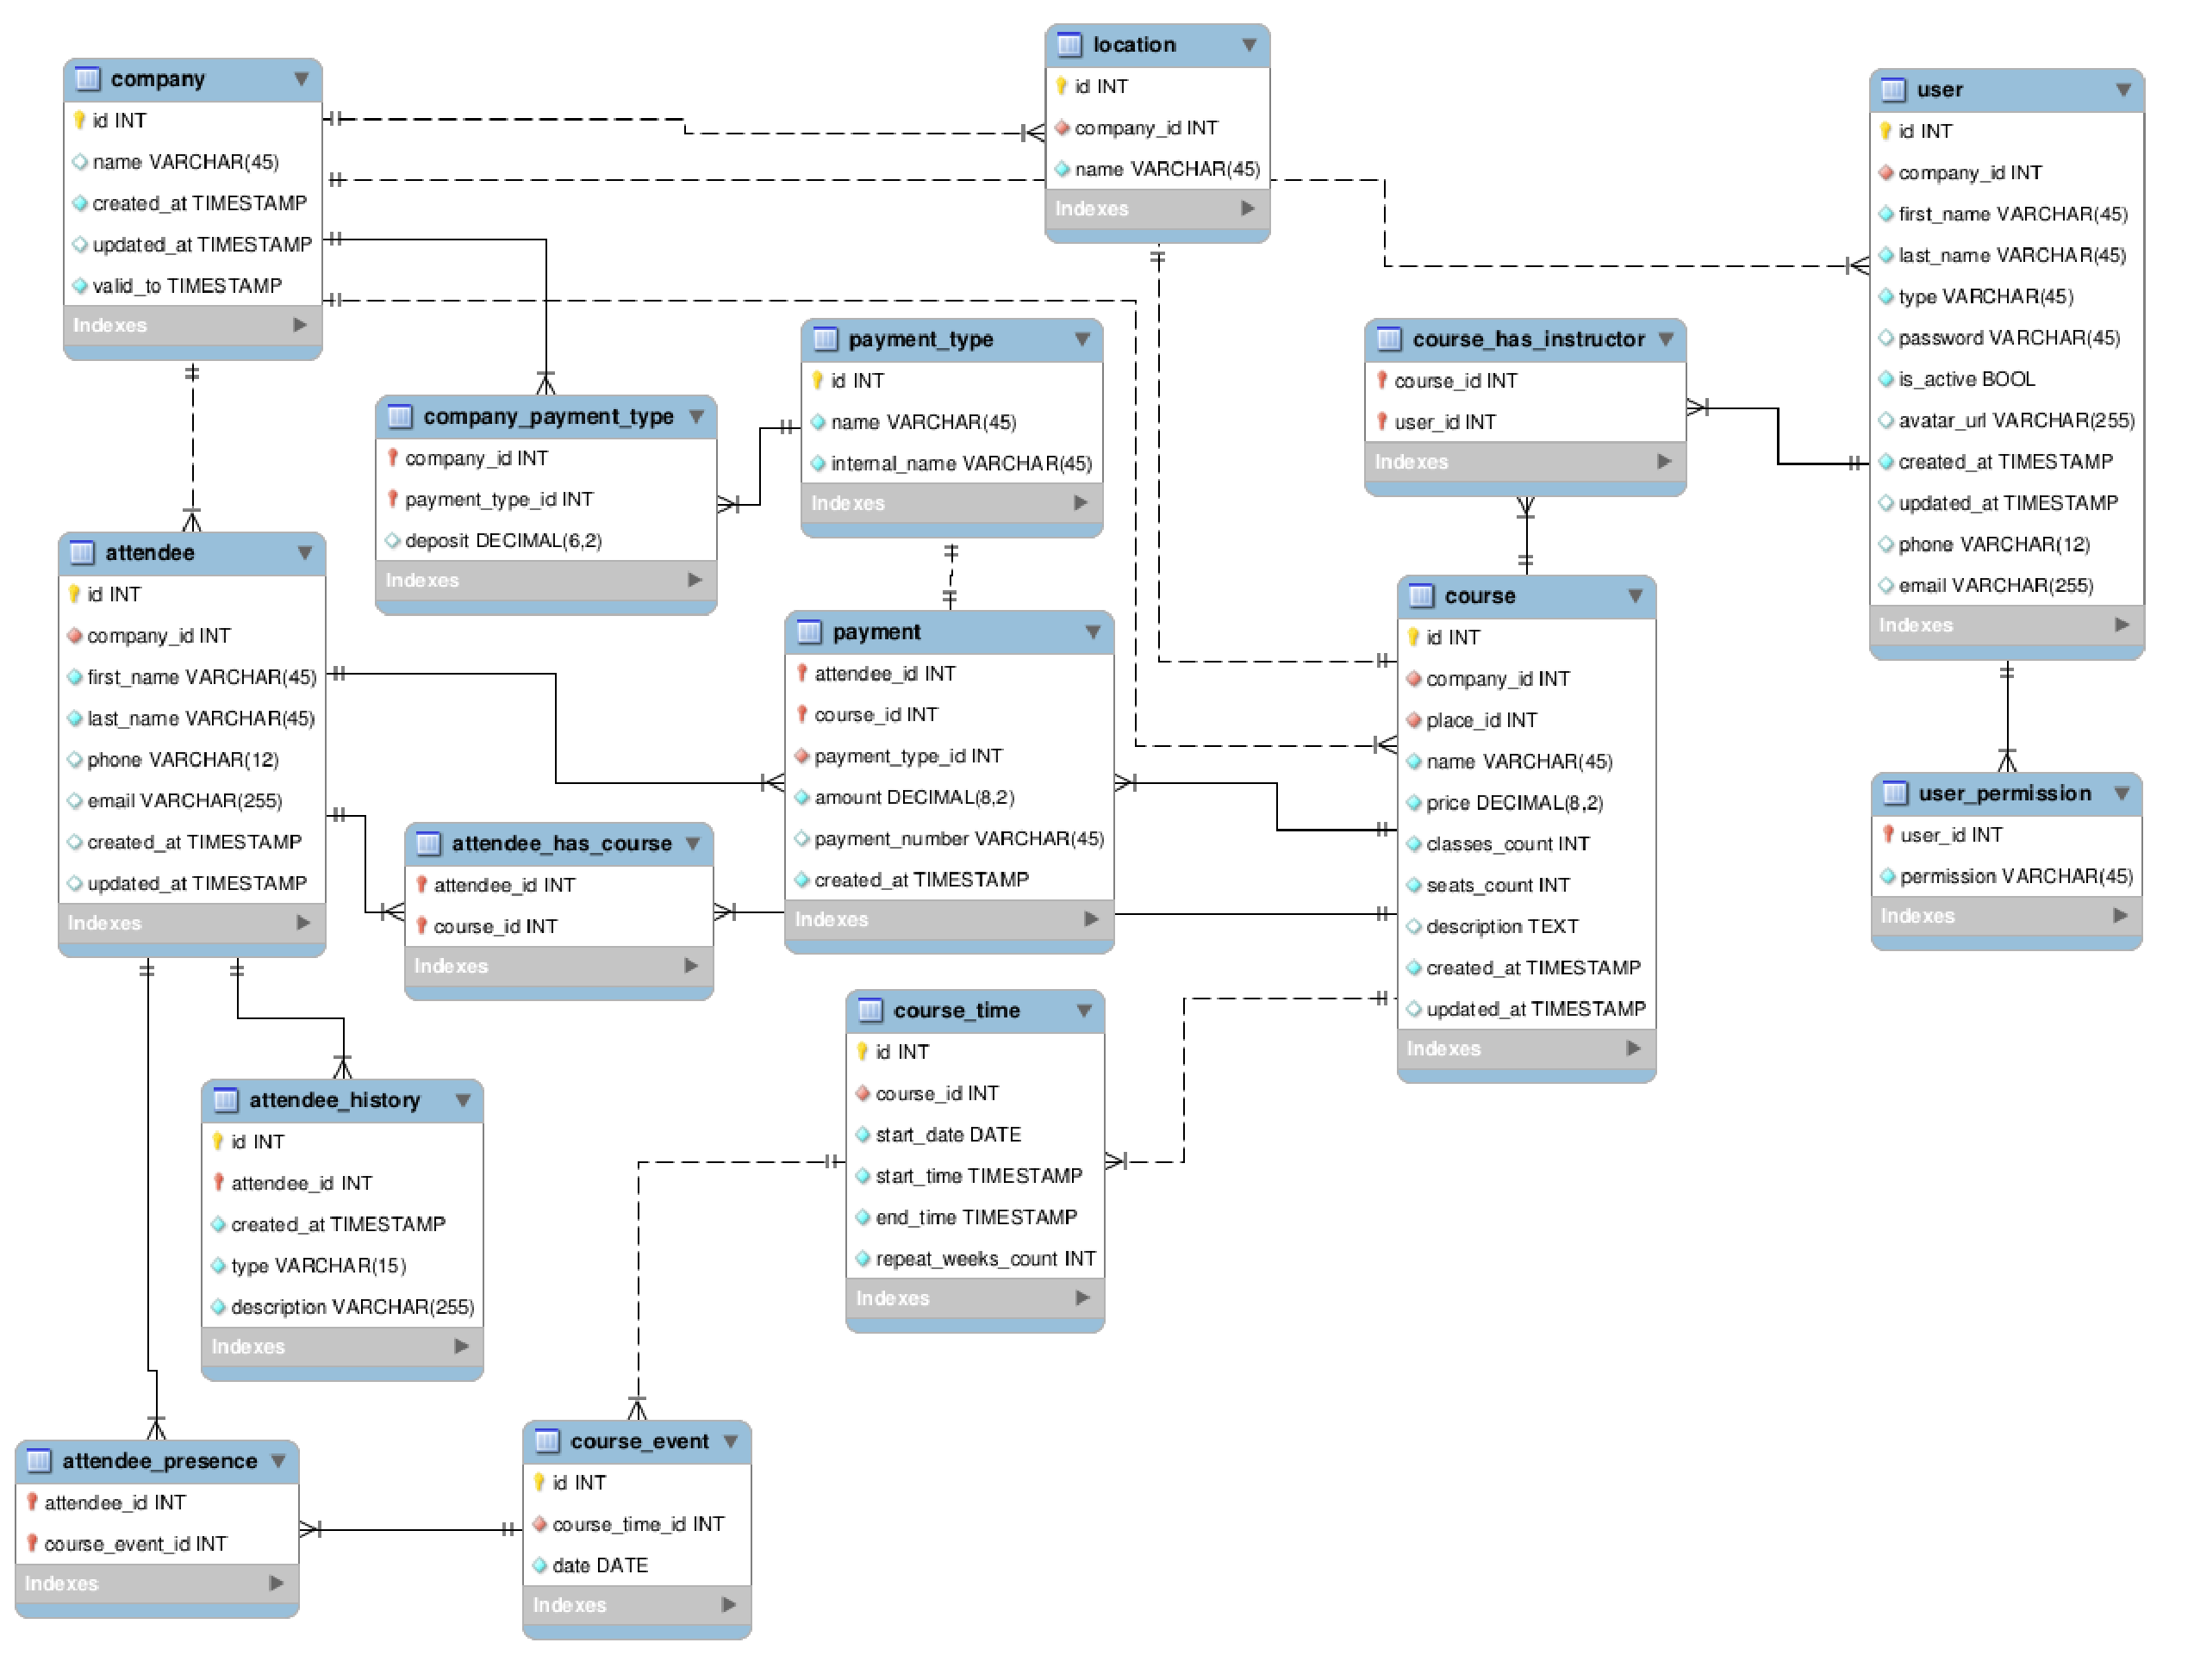
\includegraphics[width=\textwidth]{schema}
    \caption{Schema of DNCR database presents relations between dance school (company), courses, attendees, payments and instructors / administrators.}
    \label{fig:schema} 
\end{figure}

Another decision has been made to use lightweight virtualization for development environment - the team used Docker containers to achieve same environment as on their server, that is Debian with Apache configured to serve both minimized Javascript front-end app and handle API calls to backend PHP app. This way, despite working on different operating systems  the whole team would have the exact same server environment with the same dependencies and versions of each library and tool. Another, very similar Docker image was used for Continuous Deployment, that is after each Pull Request tests were launched inside Docker image using Shippable DevOps platform, in order to ensure that application didn't break in some unexpected way.

For easy collaboration, the team initially used Asana, but after a month switched to Trello to manage amount of work in progress (WIP) via Kanban board. For Git, private GitHub repository was used and all the tools were integrated with instant messaging tool - Slack.

\subsection{Next months - focus on implementation}
Having made market research to gain confidence in initial direction and having made technological decisions and developer environment all set up, in late July the team decided to focus all efforts on implementation in order to have MVP ready for October.

\begin{figure}[h]
    \includegraphics[width=\textwidth]{gui-sketch}
    \caption{Low fidelity GUI sketch presenting calendar and selected course in single view}
    \label{fig:gui-sketch}
\end{figure}
\begin{figure}[h]
    \includegraphics[width=\textwidth]{gui-balsamic}
    \caption{High fidelity GUI prototype using Balsamic program, same view as presented in Figure \ref{fig:gui-sketch}}
    \label{fig:gui-balsamic}
\end{figure}
\begin{figure}[h]
    \includegraphics[width=\textwidth]{gui-placeholder}
    \caption{Actual application in Angular, same view as in Figures \ref{fig:gui-sketch} and \ref{fig:gui-balsamic}. TODO insert actual screenshot later}
    \label{fig:gui-angular}
\end{figure}

\subsubsection{Mockups and GUI vision}
A very important aspect of the project was Graphical User Interface (GUI), because one of main problems it was solving was manual and repetitious actions needed to be performed by dance school receptionist - the team was aiming to make them easy and convenient. From the beginning it was clear that interface would evolve around some view of calendar. At first the team discussed the GUI using low-fidelity sketch on paper, and then, for implementation reference, as well as for GUI validation with the client, high-fidelity GUI prototype was prepared using Balsamic program. Figures \ref{fig:gui-sketch}, \ref{fig:gui-balsamic} and \ref{fig:gui-angular} present the same view evolution from low-fidelity sketch to actual application.

\subsubsection{Meeting with client and design validation}
On 12th of August the team representatives met with client to verify created design. The client was shown interactive prototype achieved using Balsamic Links, that is buttons on static wireframes linked to another static wireframes, producing the illusion of full interactivity. The client enjoyed the prototype and was satisfied with the simplicity of design. He then proposed various additional features to be added in later phase of the project - different client types and award system (features from loyalty program software he was acquainted with), integration with his school's website, attendance visualization and checking attendance via QR-codes or special electronic card. After discussion we agreed that after MVP is done those features would be definitely revisited.

% \FloatBarrier
\subsubsection{Collaboration model}
The team decided that all 6 developers on the team would be working ``full-stack'', that is both on back-end and front-end side of the app in order for each developer to have sufficient autonomy to quickly implement full business features. As mentioned earlier, only one developer was previously acquainted (and in his case, proficient) with used technologies. The team accepted initial slow-down for everyone to catch-up with technologies (whose main choosing criteria was ease of learning) and predicted to gain traction after few weeks.

As most of the team worked only part-time on the project and the team naturally did not have dedicated workplace for their needs at that point, 4 team members agreed to work daily in the morning at agreed time before work - 7:00 a.m., while two others preferred little later time. The goal was to minimize feedback-loop between team members, so each question / interaction / review wouldn't have to wait a few days for response, unnecessarily prolonging each task completion. Moreover, the team decided to meet every month to discuss progress, areas to improve and general direction and strategy.

\subsubsection{August - implementation progress}
In August first features started to appear:
\begin{itemize}
\item Login page
\item Initial, basic version of landing page to promote product
\item Basic manager (admin) and receptionist views
\item Adding new attendees
\end{itemize}
Furthermore, database schema was created and online payment intermediaries research was performed in order to include ability to pay for courses online.

By this time it became clear that working remotely proved to be a bigger challenge than the team expected - only 2 members worked regularly each morning as was agreed on and 2 members didn't make progress on any task.

\subsubsection{September - implementation progress}
Features implemented in September:
\begin{itemize}
\item Login authentication
\item Attendees list
\item Adding dance instructors and instructors list view
\item Calendar component presenting courses
\end{itemize}
It's worth noting that all of mentioned tasks had very broad definition of done - each task included front-end and back-end validation, handling different sizes of display (via Bootstrap framework responsive capabilities), and even elegant back-end internationalization, which resulted in very long implementation and review periods - some tasks were implemented few weeks and then reviewed few additional weeks.

It started to become clear, that MVP by October is out of the question - the team decided to focus less on polishing the product and instead create more granular tasks, so new features could be added more quickly. Another enthusiastically received idea was to create ``hackatons'', that is long whole-team programming sessions, where 1 technology experienced developer would coach others during their work.

\subsubsection{October - implementation progress}
October progress:
\begin{itemize}
\item Dance course creation
\item Attendee details / profile view
\item Authorization improvement - automatic token refreshing so user is not logged out during application usage
\end{itemize}

Despite discussion on too long task implementation period in previous month, in October the problem became even worse due to even less regular working schedule and it was hard to schedule ``hackatons''. Consequently, motivation was plummeting and team members were clearly not spending promised amount of work on project. Intervention was needed, and so to improve work consistency and motivation, the team decided to log worked hours and change ad-hoc ``Stand-ups'' (officially called ``Daily Scrum Meetings'' held to summarize work progress and discussion of eventual impediments) to obligatory weekly ``Stand-ups'' where each team member would present their weekly work log.

\subsubsection{November - implementation progress}
\begin{itemize}
\item Multi-tenancy - application could now handle multiple dance schools 
\item Added payments - receptionist can insert attendee payment with one of several available methods
\item Application-wide notifications
\item Email sending to attendees
\item Visual indication of attendee payment status
\item Dance course editing and handling multiple course times
\end{itemize}
As features implemented in November might indicate progress, but in fact most of them was just a result of implementation effort during October. In November feature-creation cycle was even longer and work-logging and weekly ``Stand-ups'' were of little help, as most members spent less and less time on a project.

\paragraph{Meeting with subject matter expert}
On 12th of November the team representative met with subject matter expert - an acquainted senior ballroom dancer who organizes dance tournaments and who is knowledgeable about targeted market and has collaborated with various dance schools. 

First part of the meeting consisted of loosely designed usability test - the expert saw the application for the first time and knowing what the application does, he was supposed to discover application capabilities by himself, without any guidance. His interaction was observed and all remarks and troubles were noted.

As a result, 18 improvements were proposed and discussed, ranging from major usability flaws like inability to add existing attendee to another dance class (GUI for adding attendee to course only allowed for creating new ones) to various features the team hasn't yet considered, but are part of schools business procedure - how to handle ``waiting lists'' when dance class reaches participants limit or someone waits for the course to start in the future? Is somebody enrolled to course only when one pays, or just when one expresses interest and gives his data? How to handle bonus visits and coupons for clients for several entries for any course? How to handle courses designed for ``pairs'' only? And many other similar aspects not previously considered.

During the second part of the meeting business model was discussed, in particular online payments viability for dance schools and due to various legal reasons (i.e. concerning fiscal evidence) this feature was decided to be postponed and substituted with plain email with reminder about due (or incoming) payments and dance schools bank account - as a easier way to validate the idea with less legal consequences.

% \subsubsection{Pivoting idea - ZnajdzTaniec.pl} % shouldn't discussion about mvp - features instead of hypothesis validation come later?
% As it was becoming increasingly clear that building what the team considered to be an MVP proved to be a long and tedious task, the worst thing seemed to be that instead of validating the idea for the business model, the team was constantly preoccupied with features. That is, after few months of development the team wasn't any more knowledgeable about whether their product would fit the market.

% Sure, the team could reach out to some more schools and show them Balsamic interactive prototype to get initial reaction and... \textbf{TODO move this section to somewhere in project evaluation and expand on this idea.}

\subsection{Decision to end the project}
After consultation with each team member about their individual reasons for constantly decreasing commitment, finally, during a meeting on 1st of December the decision has been made to end the project. The team decided to open-source the code on GitHub (\url{https://github.com/tlegutko/dncr}), the client would be proposed to evaluate competitive software and the team did ``Project Retrospective'' to discuss what went well and what were the lessons learned.

The team's December discussion is presented in Section \ref{sec:dncr-proj-eval} as the beginning of project evaluation.

\section{DNCR project evaluation}
\label{sec:dncr-proj-eval}
This section starts with project evaluation performed by the whole team on the day when project ended and continues with answers to research questions specified at the end of Section \ref{sec:probl-form-meth}.

\subsection{DNCR retrospective meeting}
The whole team met 1st of December and made the decision to end the project. Then the team proceeded to ``project retrospective'' in order to discuss strengths and weaknesses of the project.

\begin{figure}[h]
    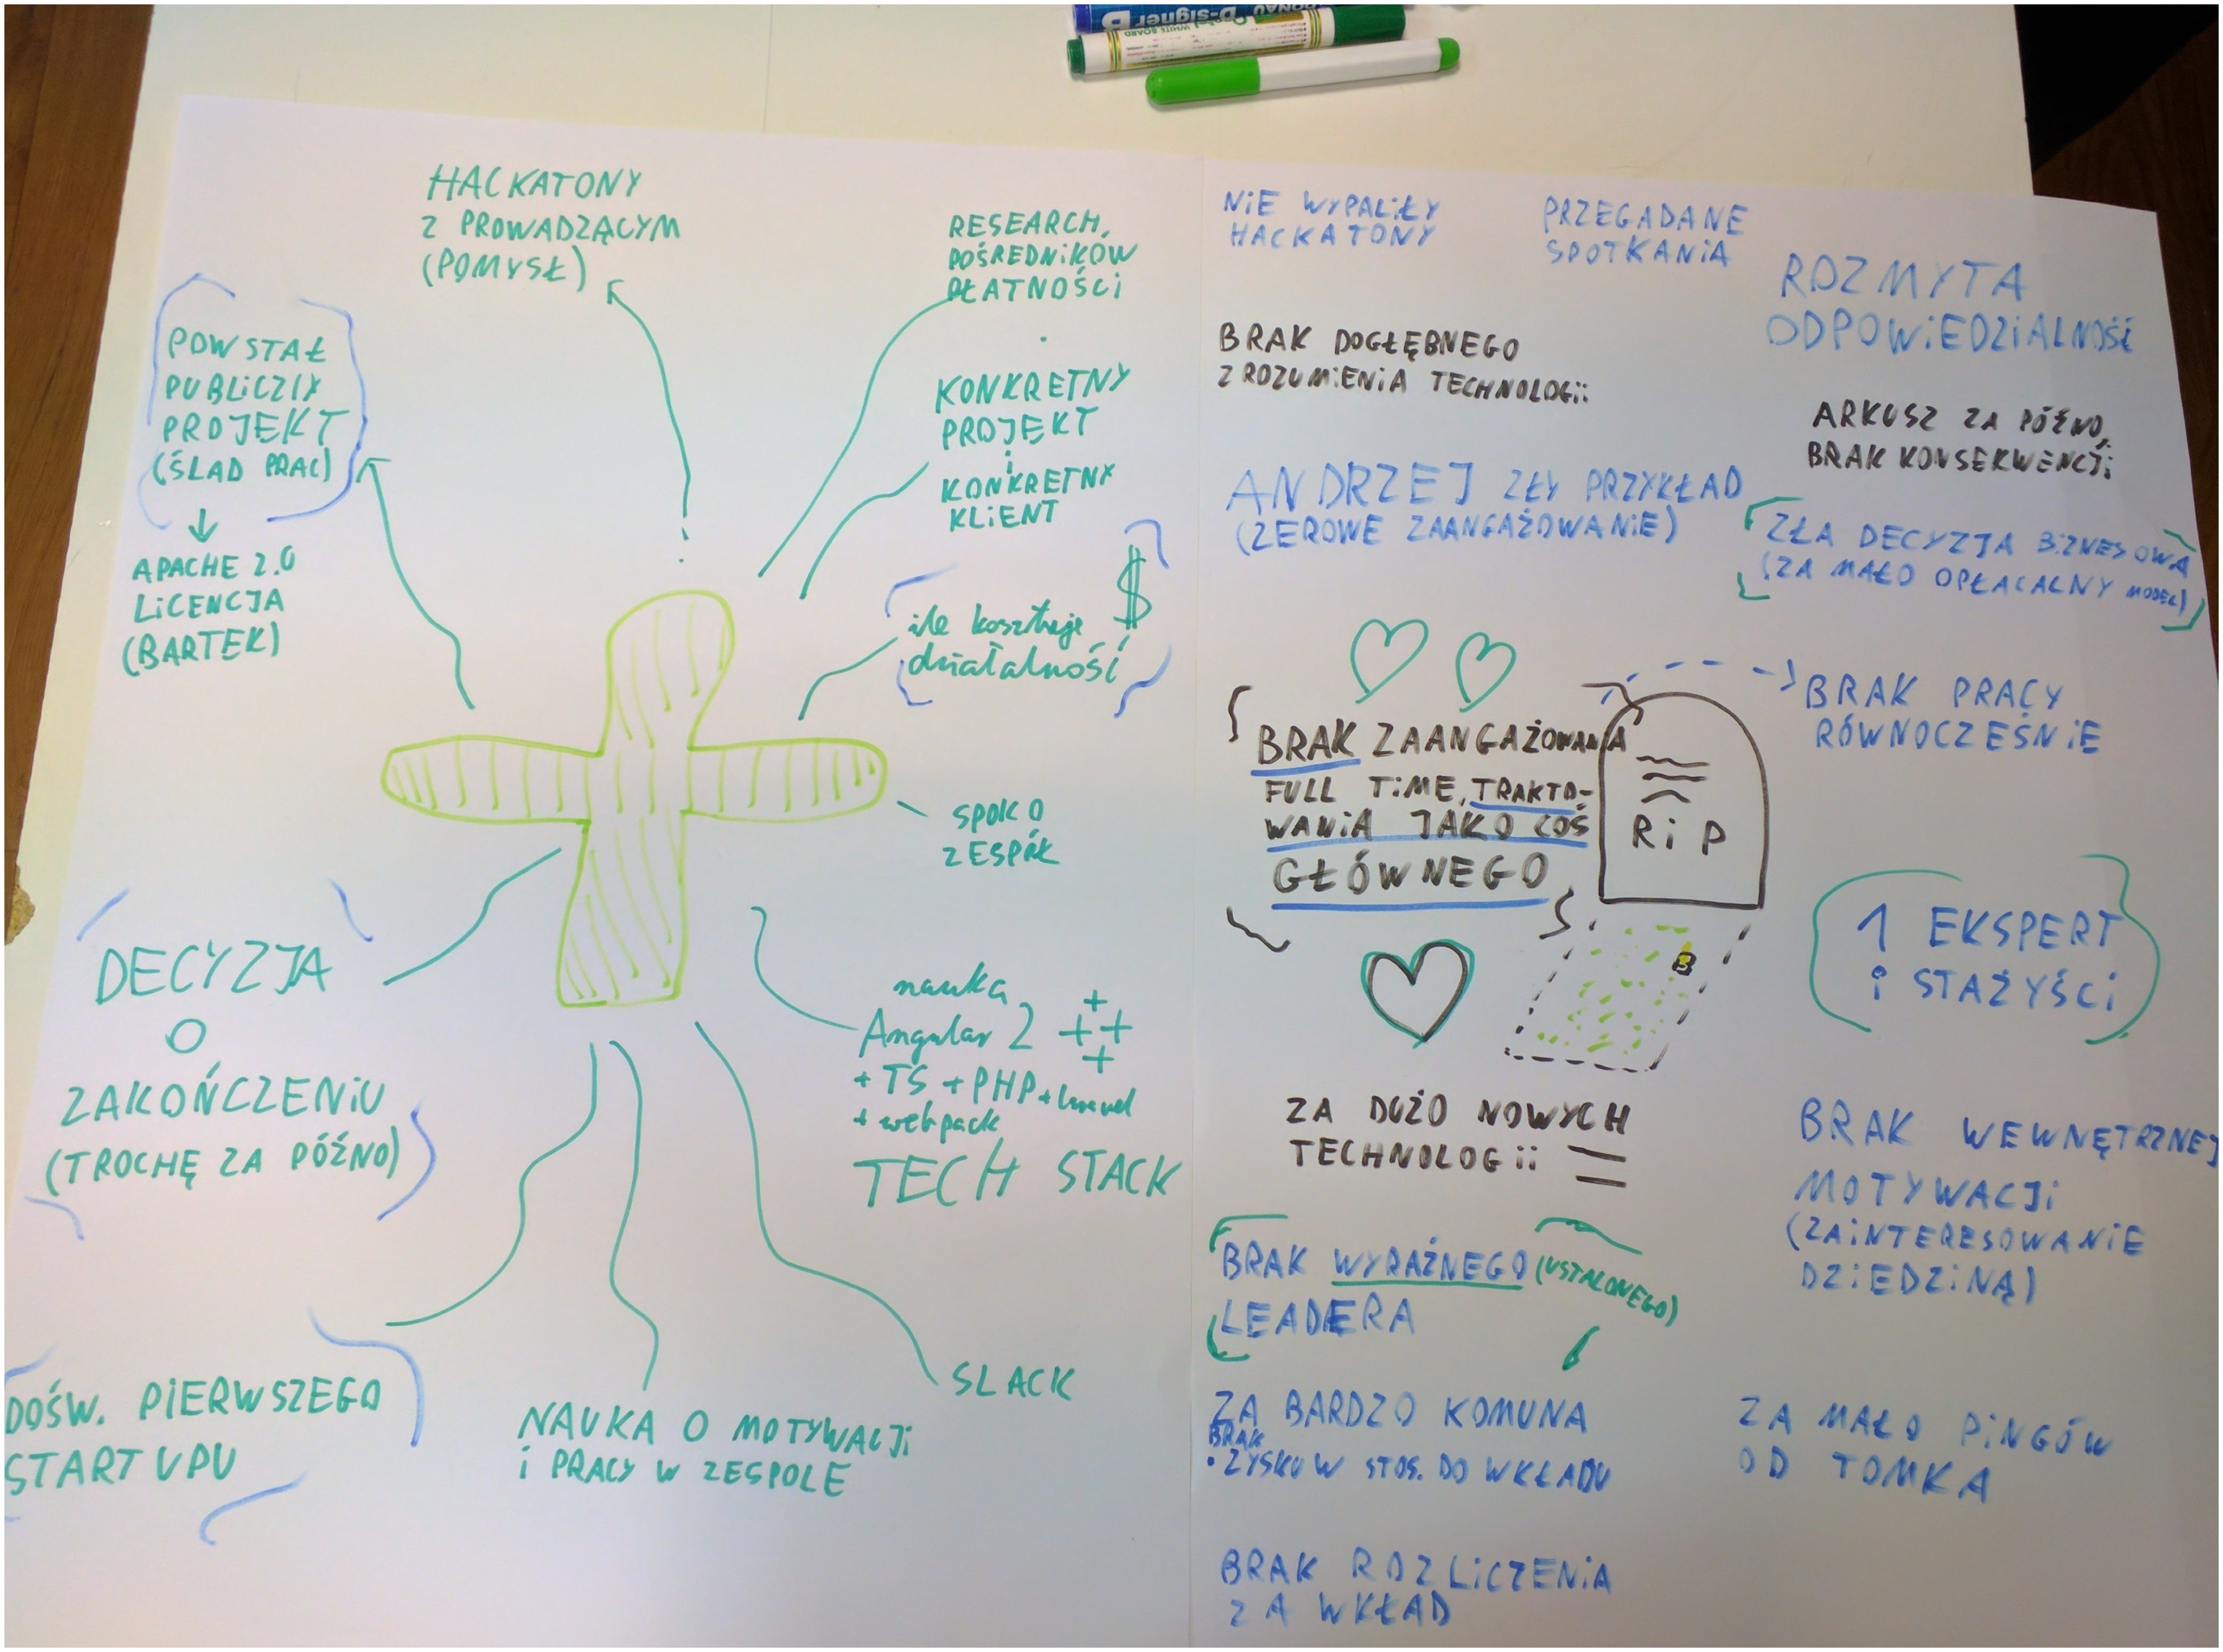
\includegraphics[width=\textwidth]{dncr-funeral}
    \caption{DNCR project summary made collaboratively by whole team during the meeting when the decision has been made to discontinue the project}
    \label{fig:dncr-funeral}
\end{figure}
\FloatBarrier

\subsubsection{What went well}

Among the positive aspects of the project the team listed:
\begin{itemize}
\item Technology stack - although many team members didn't manage to become productive in it, it was drastically different experience from what most of them used daily at work and allowed them to learn a lot
\item Experience of first startup, as it often takes several failed attempts before successful one
\item Learning about many legal and financial aspects, how much it costs to sustain private firm, how much it costs to start limited liability company and what are the best options when using online payments intermediaries
\item Swift, albeit slightly too late decision to end the project when it became clear it wouldn't lead anywhere. Also the fact that project was rather well defined and had client from the start, so the initial goal was clear.
\item The team enjoyed collaborating together and working on project outside paid work allowed them to learn a lot about aspects of team motivation. The team appreciated various methods that were attempted to make collaboration work (retrospectives, idea for guided hackatons, work logging and others)
\item Open-sourcing the project, which leaves public trace of performed work, which can be very useful, i.e. can be added to CVs.
\end{itemize}

\subsubsection{What made the team fail}
The team found the following reasons for project failure:
\begin{itemize}
\item The main, most important reason was that most team members didn't treat the project as their ``main thing'' they needed to focus on. On one hand it's hard to expect several people to suddenly resign from their work and spend all their efforts on project that might or might not succeed and might or might not return the invested time and money, on the other hand if something is not given appropriate priority, then naturally regular work and other aspects will at times consume most of attention and commitment to side project will plummet. And with very little time spent on project, there are very few mistakes to make in order to still have chance for success.
\item Overwhelming technologies and ``one expert surrounded by interns'' situation. It's natural to learn new languages, frameworks and tools in software development, but launching into two completely unfamiliar technology stacks, especially if one of them is front-end development, which in last years became quite daunting for newcomers. Another aspect of technological shortcomings was usage of Docker in development environment, which in theory works on all platforms, but in practice broke constantly with new versions for team-members working on Windows. Overall, as was listed during the meeting, ``lack of in-depth technology understanding'' naturally resulting from lack of experience with technology slowed most of team-members down tremendously.
\item Next critical aspect was about the way the team organized work and responsibility among team members. On the project kick-off meeting the team decided that despite different skill-sets (1 experienced developer) and different amount of spent time (1 developer worked on DNCR full-time), work of every member would be treated equally in light of future financial gains. On top of that, there was no clear leader elected and so instead of enthusiastic, collaborative atmosphere, team members demonstrated sociological phenomenon called diffusion of responsibility.
\item Diffusion of responsibility was amplified by lack of consequences towards underperformers. Out of 7 initial members, one resigned early and two other practically didn't contribute anything during the course of whole undertaking. One other was active mostly in first phase and as a result only 3 people worked for declared amount of time, and seeing lack of engagement from others only lowered morale and enthusiasm of active members. 
\item Another aspect of low commitment among team members was lack of intrinsic motivation. Only one member knew the client directly and felt close to the domain and emotionally invested to make the project succeed, others had more cold, business oriented attitude. And as there was also no team leader, those members felt they weren't held accountable for keeping constant commitment.
\item Many team members confessed to be discouraged over time by initial idea for business model, claiming that number of dance schools on the market is not enough to financially return the investment any time soon and that bringing application to another domains or creating platform for dance class attendees was too far in the future.
\item Another set of drawbacks was that many ideas to improve team workflow didn't work out - guided hackatons didn't take place after all, work log was introduced too late and meetings were mostly about business and discussion, not about coding sessions. Lack of regular work in one place was in itself mentioned as important aspect - it made it harder for underperformers to gain traction and it made collaboration, especially code reviews, much more time consuming.
\end{itemize}

\subsection{Study results}
\label{sec:research-questions}
Few months later, writing this thesis, the author has acquainted himself with work of many authors on related topics in order to understand more deeply not only why did the project fail, but what could have been done differently. What other approaches could facilitate collaboration and improve chances of success of future projects and what advices could be directed towards other startups. And so, with benefit of hindsight, the following is author's answer to research questions.


\subsubsection{RQ1: What Lean UX practices are most important in beginning phases of startup?}
Early stages of startup activities revolve mainly around validating problem, market and the product \cite{klein2013ux}. DNCR team did quite well in that regard, performing both qualitative and qualitative market research and doing competitive product audits. On top of that, design of product was validated with client using interactive prototype. All those activities gave the team necessary confidence in initial direction of action.

Of course there was room for improvement - hypothesis that customers would want to search for dance courses and pay for their classes online was critical for product future, yet instead of performing semi-statistically significant (40 respondents) online survey, it would be better to follow Steve Blank \cite{blank2013four} advice of Getting Out Of the Building (GOOB) and just go to some dance courses and perform survey in person, so follow-up questions could be asked, which would be a much better way to validate the idea.

Furthermore, more dance schools should be collaborated with from initial phases of the project, so solution the team would arrive to would be more universal and not just a perfect fit for first client. The team was well aware of that, but planned to acquire new clients after initial MVP version, which unfortunately didn't work well as the team failed to finish MVP.

The general advice for startups is then to:
\begin{itemize}
\item Actually perform various types of research and design validation before starting implementation, as it allows to clearly set initial direction
\item Especially in the beginning, focus on in-person, qualitative surveys. Quantitative research has it's many uses, but as Laura Klein \cite{klein2013ux} notes, online surveys cannot be considered as being in touch with users.
\item Competitive products audits cannot be recommended enough. They let the team learn from mistakes of others and in case of EU markets, often very similar solution already exists abroad (especially in US) an can serve as great source of inspiration.
\end{itemize}

\subsubsection{RQ2: How can Lean UX practices influence Minimal Viable Product building and what are impediments in adopting them?}
As for implementation, Lean UX, following Lean Startup, advices treating each feature as a hypothesis to be tested and considered done only once proved to improve business metrics, usually via quantitative A/B testing. This can be hard at early implementation stages, when there is neither infrastructure nor user base for such tests yet, so in order to start iterative build-measure-learn loop, the team has to swiftly create Minimal Viable Product. It's important to note that Lean UX doesn't really discuss or define practices for MVP building, it generally embraces Agile and assumes the engineers will do the right thing. Laura Klein \cite{klein2013ux} discusses how hard is it to choose just the most necessary features at the beginning.

And this is where DNCR team failed hard. Initial design vision and ``minimal feature-set'' was ridiculously misaligned with team skill-set and it was noticed very late in the process. As a result, after more than 4 months focused solely on implementation in team of 6 developers, the MVP still wasn't officially finished. Eric Ries \cite{ries2011lean} addresses this in his case study of actions by David Binetti, the CEO of Votizen, platform for civic participation in political process:
\begin{quote}
Votizen story exhibits some common patterns. One of the most important to note is the acceleration of MVPs. The first MVP took eight months, the next four months, then three, then one. Each time David was able to validate or refute his hypothesis faster than before. 
\end{quote}
Ries then argues that it's not due to Binetti previous product development work, as it often was discarded across different MVPs. It was partly due to existing testing infrastructure, but it was mostly due to ``hard-won lessons David had learned through each milestone''.

So it's not only the DNCR team that misunderstood the minimalism intended by MVP. In particular, the team needlessly focused on correct design scaling based on resolution - mobile first approach is a great guideline, but it just wasn't needed at this point in time. Moreover, team members were too strict in code review process - good code is important, but when reviews take long weeks and slows feature development, then it's a waste of effort. When learning new technology it's okay to have less quality code and improve later. It's infinitely better to have validated product ridden with technological debt than to have quality code that didn't reach the market or even validation phase. Ideally, it's great to have both, but sometimes the choice has to be made.

Thus, general advice for startups regarding MVP is to:
\begin{itemize}
\item Consider team skill-set and other performance risks when determining feature-set of an MVP. It's main role is to quickly enable build-measure-learn loop and until it starts, the team doesn't really learn anything about their product.
\item Prioritize, prioritize, prioritize, as sometimes too much emphasis on good development practices are a waste of effort. Laura Klein \cite{klein2013ux} even proposes to put off visual design at first, as it is both faster to iterate and it doesn't influence interaction testing.
\item Consider MVP to be more of a prototype than a product. MVP has to be viable, but the minimal part is really important - if developers don't feel shame about lack of features of released version, or worse, haven't released any version few months into development, then this is not MVP.
\end{itemize}

\subsubsection{RQ3: What are most essential advices for startups regarding technology?}
This question is very hard to answer other than ``it depends'', as every startup faces different technological challenges.

Firstly, it's important to really understand consequences of technological choices. In DNCR project, choosing backend technology language Ruby was considered and eventually PHP was chosen despite the fact that most of the team had extensive experience in Java. Of course it's true that Java servers cost more and of course it's tedious to always use the same language and technology, but startups really provide enough novelty outside of technology and cost of leaving familiar technology stack for new one is really not to be underestimated. As almost all members were also new to front-end development, so instead of being productive at least in server-side aspects from day one, many members failed to become productive at all during the project.

Secondly, in principle it's great to have whole development team consisting of only full-stacks, it doesn't unnecessarily split the team and every member has autonomy to implement full business features on their own. In practice, it resulted in low granularity tasks that took weeks to implement and additional weeks to review.

Moreover, Docker as a tool of abstracting over developer environment is great in theory, but in practice it made three Windows 10 developers lives in the team miserable, crashing constantly in hard to debug ways. Two of them switched to Linux Virtual Machines and one suffered with broken environment after each update to the end of project. Additionally, development environment facilitating Docker prevented the team from being able to use Angular HMR (Hot Module Reloading), which would make development feedback loop even tighter.

Another aspect was decision to use Release Candidate version of Google's Angular, before it's 2.0 release. In theory release candidates, made after alpha and beta, should be stable, but was not the case, Angular upgrades around RC5 were painful, as Google team introduced significant breaking changes and updated their documentation which wasn't versioned before 2.0 and DNCR team couldn't upgrade because of dependencies on earlier Angular RC versions. And for some time the team was out of sync with documentation.

Yet another aspect was implementing token authorization and in general user login handling. The team evaluated using COTS (Commercial Off-The-Shelf) solution, offering Social Sign-In for free until certain user limit, but eventually the team decided to manually implement solution using JWT (JSON Web Tokens). Again, in this case it might've been a better choice to just use COTS solution and worry later once product is validated and number of users approaches that limit.

The team, of course, did some things well too - one of them was to start implementation phase from extensive documentation about development environment setup, integration with IDE and configuration of Continuous Integration and so that important aspect went smoothly (this setup documentation is available at \url{https://github.com/tlegutko/dncr}). Usage of Docker was the only part that didn't go well.

Overall, general advice for startups regarding technology is to:
\begin{itemize}
\item Think twice before relying on Docker when using Windows
\item Above all, think ten times before choosing novelty of unfamiliar technologies and seriously consider its impact on team's productivity
\item Full-stack development team is nice, but consider that an end-goal, not a requirement from day one. It's okay to specialize in the beginning. And keep high enough granularity of tasks.
\end{itemize}

\subsubsection{RQ4: What are most essential advices for startups regarding team?}
As mentioned during project retrospective, the team suffered from diffusion of responsibility due to underperformers and lack of leadership.

Regarding leadership, the team had three candidates: leader of team at work where most developers collaborated prior to project, developer who brought the idea along with the client and organized team's work and the only developer experienced with technologies, who was also responsible for design. The first one wasn't very committed from the start, while the second and the third thought the other one was more fitting. The end scenario was worst possible, as no one was selected and it negatively affected perceived responsibility of team members.

Lack of formal definition of startup \cite{paternoster2014software} was another reason for lack of leadership and even distribution of costs - one of leader candidates perceived a startup as a collaborative, passionate effort where there is no need for formal structure and everyone gives their all. As Giardino et. al. \cite{giardino2014early} notice:
\begin{quote}
  One of the key determinants of success in startup companies is the passionate behavior of the founders. People who lack passion often use the first barrier they encounter as an excuse for failure. People who have high passion will do whatever it takes to overcome those barriers.
\end{quote}

This assumption was part of the reason that underperformers' behavior was accepted for so long. Initially no formal structures were assumed to be necessary, as team was doing well on initial motivation from starting the project. Furthermore, initial lack of productivity was expected due to lack of experience with technology. What was noticed much too late was that lack of productiveness was not due to hardships in mastering technology, it was due to not spending time on the project. Work logging and simple performance evaluation like weekly summary should have been introduced and acted on earlier.

Moreover, the team lacked regular face-to-face collaboration, especially during implementation. Even though it's one of main principles listed in Agile Manifesto, the team failed to incorporate it. Of course it's hard to coordinate 6 people, mainly working after regular work hours, of course it's more convenient and flexible for developers to work remotely when it fits them most. But the truth is, if the team is inexperienced with technology, there is a high chance that this will not work. Firstly, every technological question and problem can either take longer when developer solves it himself or can be solved instantly with help of someone more experienced. The former is of course necessary for effective, long term learning, but lack of balance between the too is of a huge impact for productivity. Secondly, all discussions, especially over code review, take much longer. And unproductive loneliness takes high toll on motivation.


Advice for startups regarding social/people/team aspect is to:
\begin{itemize}
\item Explicitly choose leaders. Choosing technological leader and team leader is a good choice in situation similar to DNCR project. Choosing another configuration is also good, as long as roles are clearly defined.
\item Although both methodological and technological advancements made startups much less risky, they still require passionate founders who will persevere and overcame all eventual roadblocks.
\item Underperformers should be moved away from team quickly. It may seem counter-intuitive, as extra developer seems to always push work a little bit forward, but when his contribution is minimal, slows the team down and negatively affects morale, it's the right thing to let them go.
\item Seriously consider the impact of abandoning regular collaborative implementation sessions and unless the team has experience working remotely in particular technology, think hard about counter-measures to save team's productivity.
\end{itemize}

\subsubsection{RQ5: What are most essential advices for startups regarding business/market?}ź
Advice for startups regarding business/market is to:
\begin{itemize}
\item Read Eric Ries' book ``The Lean Startup'' \cite{ries2011lean}, it's more than excellent advice on this matter.
\end{itemize}

\subsubsection{RQ7: What are most essential advices for startups regarding stuff from success factors?}
i

\subsubsection{DNCR team was not the only one with those problems}
(Why early startups fail, Applying Lean Startup: Experience Report

\section{Conclusion}
\subsection{Future work}
\begin{itemize}
  \item Software startup is not only about software, it's also about legal aspects, acquiring funding, marketing - it's still not explored in literature
  \item Still little synthesized experience report on startups (especially those failed)
  \item Metrics on tracking progress in early phases of startup (MVP building), before having clients to perform usability tests / cohort analysis and so on.
  \end{itemize}
\newpage
\listoffigures
\bibliographystyle{plain}
\bibliography{masters-thesis} 
\end{document}